\section{keyboard.cpp File Reference}
\label{keyboard_8cpp}\index{keyboard.cpp@{keyboard.cpp}}


{\tt \#include \char`\"{}keyboard.h\char`\"{}}\par
{\tt \#include \char`\"{}keyboard.moc\char`\"{}}\par


Include dependency graph for keyboard.cpp:\begin{figure}[H]
\begin{center}
\leavevmode
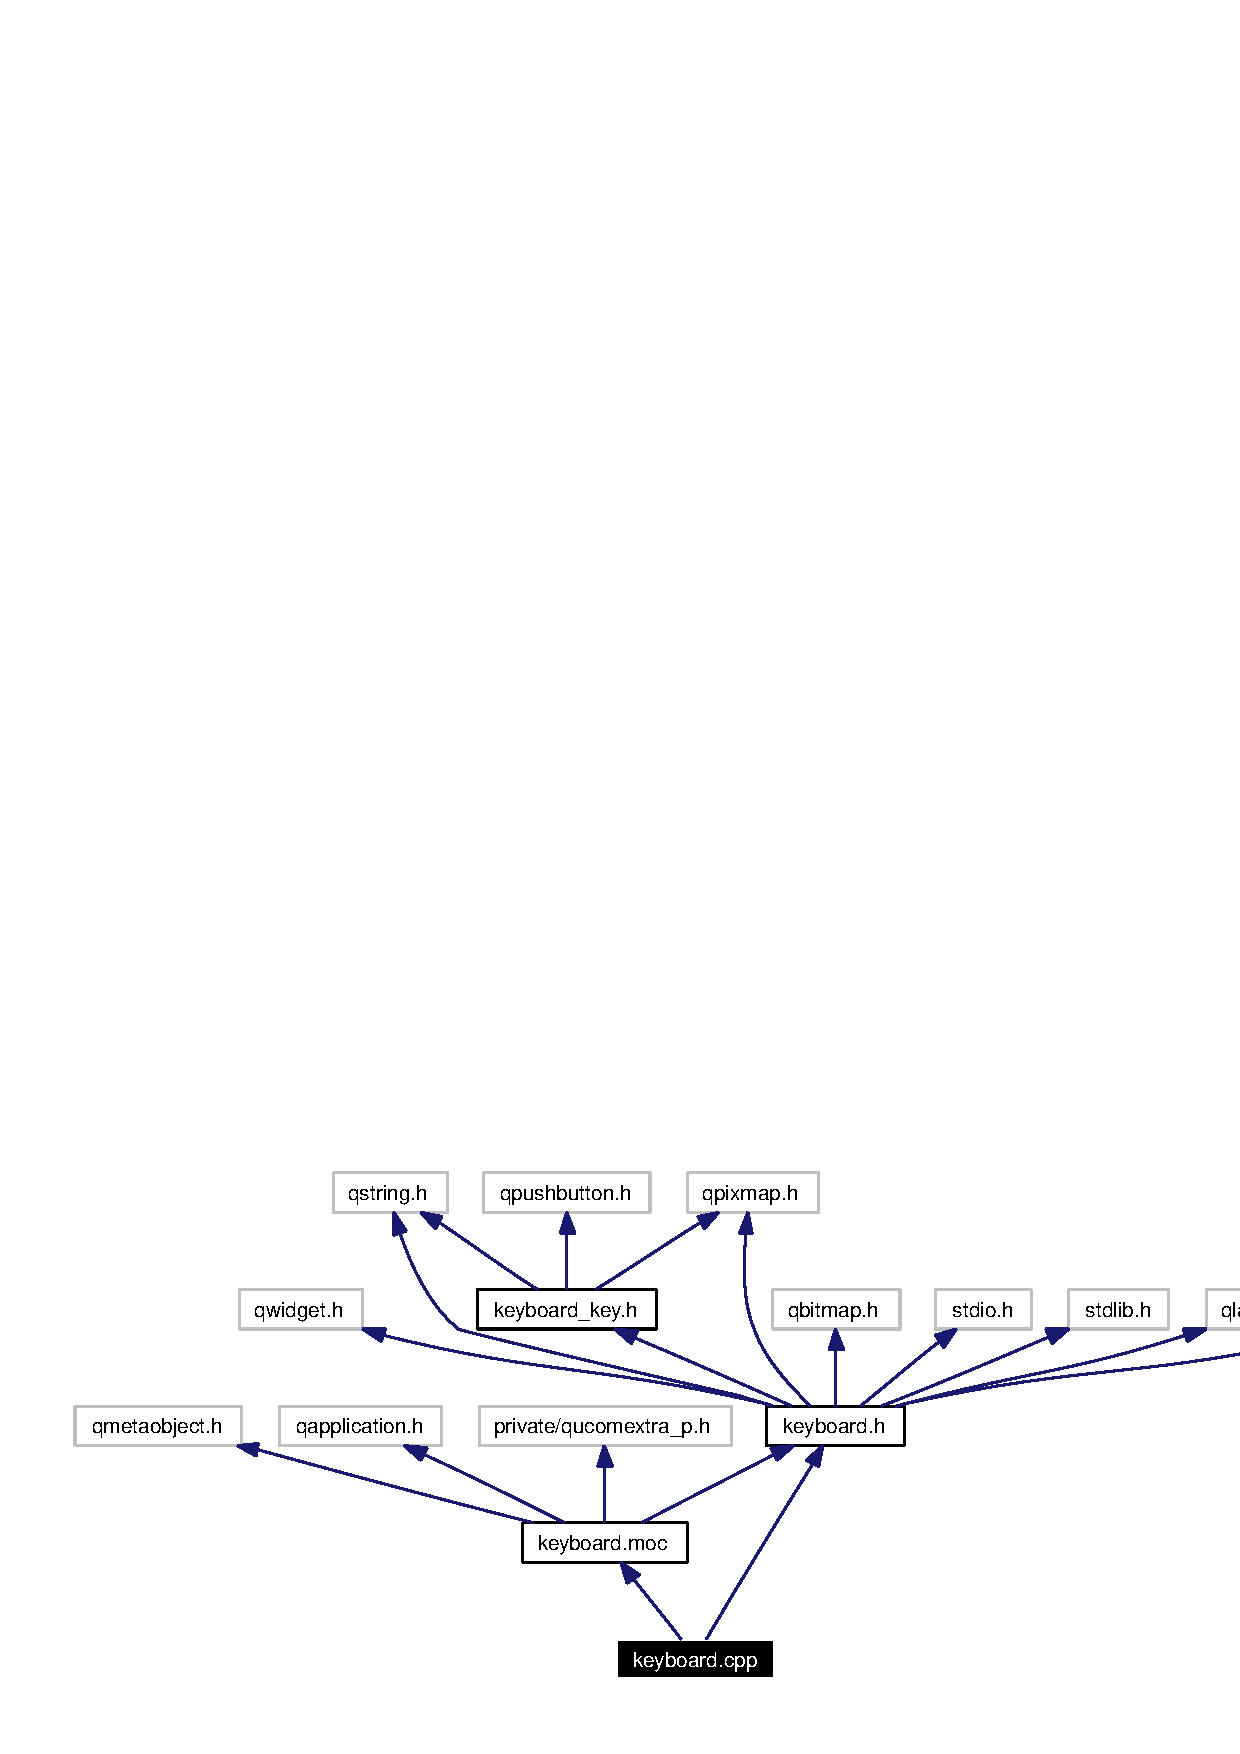
\includegraphics[width=351pt]{keyboard_8cpp__incl}
\end{center}
\end{figure}
\subsection*{Defines}
\begin{CompactItemize}
\item 
\#define {\bf KEYNUMS}\ 41
\end{CompactItemize}
\subsection*{Variables}
\begin{CompactItemize}
\item 
int {\bf Key\-Pos} [KEYNUMS][2]
\end{CompactItemize}


\subsection{Define Documentation}
\index{keyboard.cpp@{keyboard.cpp}!KEYNUMS@{KEYNUMS}}
\index{KEYNUMS@{KEYNUMS}!keyboard.cpp@{keyboard.cpp}}
\subsubsection{\setlength{\rightskip}{0pt plus 5cm}\#define KEYNUMS\ 41}\label{keyboard_8cpp_a0}




Definition at line 21 of file keyboard.cpp.

\subsection{Variable Documentation}
\index{keyboard.cpp@{keyboard.cpp}!KeyPos@{KeyPos}}
\index{KeyPos@{KeyPos}!keyboard.cpp@{keyboard.cpp}}
\subsubsection{\setlength{\rightskip}{0pt plus 5cm}int {\bf Key\-Pos}[KEYNUMS][2]}\label{keyboard_8cpp_a1}




Definition at line 23 of file keyboard.cpp.

Referenced by keyboard::Init\-Key().